\documentclass[12pt,a4paper,twoside]{article}

%------------------------------ encoding
\usepackage[utf8]{inputenc}

%------------------------------ page layout
\usepackage[left=3cm,right=3cm,top=3cm,bottom=2cm]{geometry}

%------------------------------ clickable toc and links styles
\usepackage{hyperref}
\hypersetup{
    colorlinks,
    citecolor=black,
    filecolor=black,
    linkcolor=black,
    urlcolor=black
}

%------------------------------ font macro
\newcommand*{\courierfont}{\fontfamily{pcr}\selectfont}

%------------------------------ references
\usepackage{biblatex}
\addbibresource{bib.bib}

%------------------------------ tables
\usepackage{tabularx}

%------------------------------ images
\usepackage{graphicx}

%------------------------------ font preferences (1) or sc
\usepackage[sc]{mathpazo} 
% \usepackage{newpxmath}

%------------------------------ comment
\usepackage{comment}

%------------------------------ title spec
\usepackage{titlesec}
\usepackage{afterpage}

%------------------------------ abstract
\usepackage{abstract}
\renewcommand{\abstractnamefont}{\normalfont\Large\bfseries}

\begin{document}

\begin{comment}
\begin{titlepage}
    \centering
    \vspace*{\fill}

    \vspace*{0.5cm}
    
    \huge ACULEI
    
    \vspace*{2.5cm}
    
    \vspace*{1cm}

    \begin{minipage}{\textwidth}
        \centering
        \begin{tabular}{ccc}
            \small \textbf{Brajucha Filippo} & \small \textbf{Dinelli Michele} & \\
            \small University of Bologna & \small University of Bologna & \\
            \scriptsize \courierfont{\href{mailto:filippo.brajucha@studio.unibo.it}{filippo.brajucha@studio.unibo.it}} & \scriptsize \courierfont{\href{mailto:michele.dinelli5@studio.unibo.it}{michele.dinelli5@studio.unibo.it}} & \\
        \end{tabular}
    \end{minipage}

    \vspace*{1cm}

    \begin{minipage}{\textwidth}
        \centering
        \begin{tabular}{ccc}
            \small \textbf{Hanna Youssef} \\
            \small University of Bologna \\
            \scriptsize \courierfont{\href{mailto:youssefawni.hanna@studio.unibo.it}{youssefawni.hanna@studio.unibo.it}} \\
        \end{tabular}
    \end{minipage}
    
    \vspace*{\fill}
\end{titlepage}

\tableofcontents

\newpage

\end{comment}

\begin{center}

\rule[0.1cm]{15.8cm}{1.5mm}
{{\Large{Aculei}}} 
\rule[0.1cm]{15.8cm}{0.1mm}

\vspace*{1cm}

\begin{minipage}{\textwidth}
    \begin{tabular}{ccc}
        \small \textbf{Brajucha Filippo} & \small \textbf{Dinelli Michele} & \small \textbf{Hanna Youssef} \\
        \small University of Bologna & \small University of Bologna & \small University of Bologna \\
        \scriptsize \texttt{\href{mailto:filippo.brajucha@studio.unibo.it}{filippo.brajucha@studio.unibo.it}} & \scriptsize \texttt{\href{mailto:michele.dinelli5@studio.unibo.it}{michele.dinelli5@studio.unibo.it}} & \scriptsize \texttt{\href{mailto:youssefawni.hanna@studio.unibo.it}{youssefawni.hanna@studio.unibo.it}} \\
    \end{tabular}
\end{minipage}

\vspace*{1cm}
    
\end{center}

\begin{abstract}    
\noindent Questo report descrive le varie fasi del processo di realizzazione di un dataset che 
raccoglie i dati di fotografie di animali scattate automaticamente da foto-trappole situate nei boschi 
dell'Umbria. Realizzare il dataset ha lo scopo di raccogliere una vasta quantità di dati, così da 
metterli al servizio di tecniche di intelligenza artificiale, al fine di raggruppare e potenzialmente 
classificare le fotografie.\\ 
Si esplorano due approcci: il primo prevede l'apprendimento non supervisionato basato su algoritmi di 
clusterizzazione, il secondo si basa invece sull'utilizzo di una tecnica chiamata \textit{zero-shot 
image classification} al fine di classificare le fotografie in base all'animale ritratto.\\ 
Negli ultimi anni la disciplina nota come computer vision ha fatto passi enormi, grazie a questa branchia 
dell'informatica è possibile manipolare dati complessi, come le fotografie, estraendo da esse conoscenza. 
Le informazioni ottenute dalle fotografie, le relazioni e i pattern nascosti che vengono identificati 
dall'intelligenza artificiale sono utilizzati per generare un'esperienza interattiva all'interno di un 
archivio fotografico chiamato \textit{aculei}. Il progetto \textit{aculei} nasce dall'idea di un 
fotografo milanese che ha posizionato varie foto-trappole automatiche nei boschi che circondano la casa 
in cui è cresciuto in Umbria. La volontà di pubblicare le fotografie e rendere l'esperienza sull'archivio 
ai-driven sono le motivazioni che lo spingono a ideare il progetto \textit{aculei}.
\end{abstract}

\section{Introduzione}
La computer vision è un campo dell'intelligenza artificiale che permette ai computer di estrarre 
informazioni e dati da immagini digitali, video e altri input visivi. Funziona più o meno come la 
vista umana, ma gli umani hanno un grande vantaggio: dispongono di anni e anni di esperienza in cui 
si sono allenati a distinguere gli oggetti \cite{ibm-comp-vision}. I computer devono fare lo stesso 
ma in molto meno tempo ricorrendo generalmente a tecniche di deep learning sfruttando una tipologia di 
reti neurali note come reti neurali convoluzionali. Sono state utilizzate diverse tecniche basate sulla 
computer vision come ocr \footnote{Ocr: optical character recognition è un termine che descrive i 
programmi dedicati al riconoscimento ottico dei caratteri in un documento} e zero-shot image 
classification \footnote{Task di computer vision per la classificazione di immagini in una determinata 
classe, senza alcun addestramento o conoscenza preventiva delle classi}.\\ 
Per realizzare il dataset di aculei è stata ampiamente sfruttata la computer vision in quanto i dati 
forniti sono più di 16000 immagini digitali che devono essere necessariamente processate da un computer.

\begin{figure}[!ht]
    \centering
    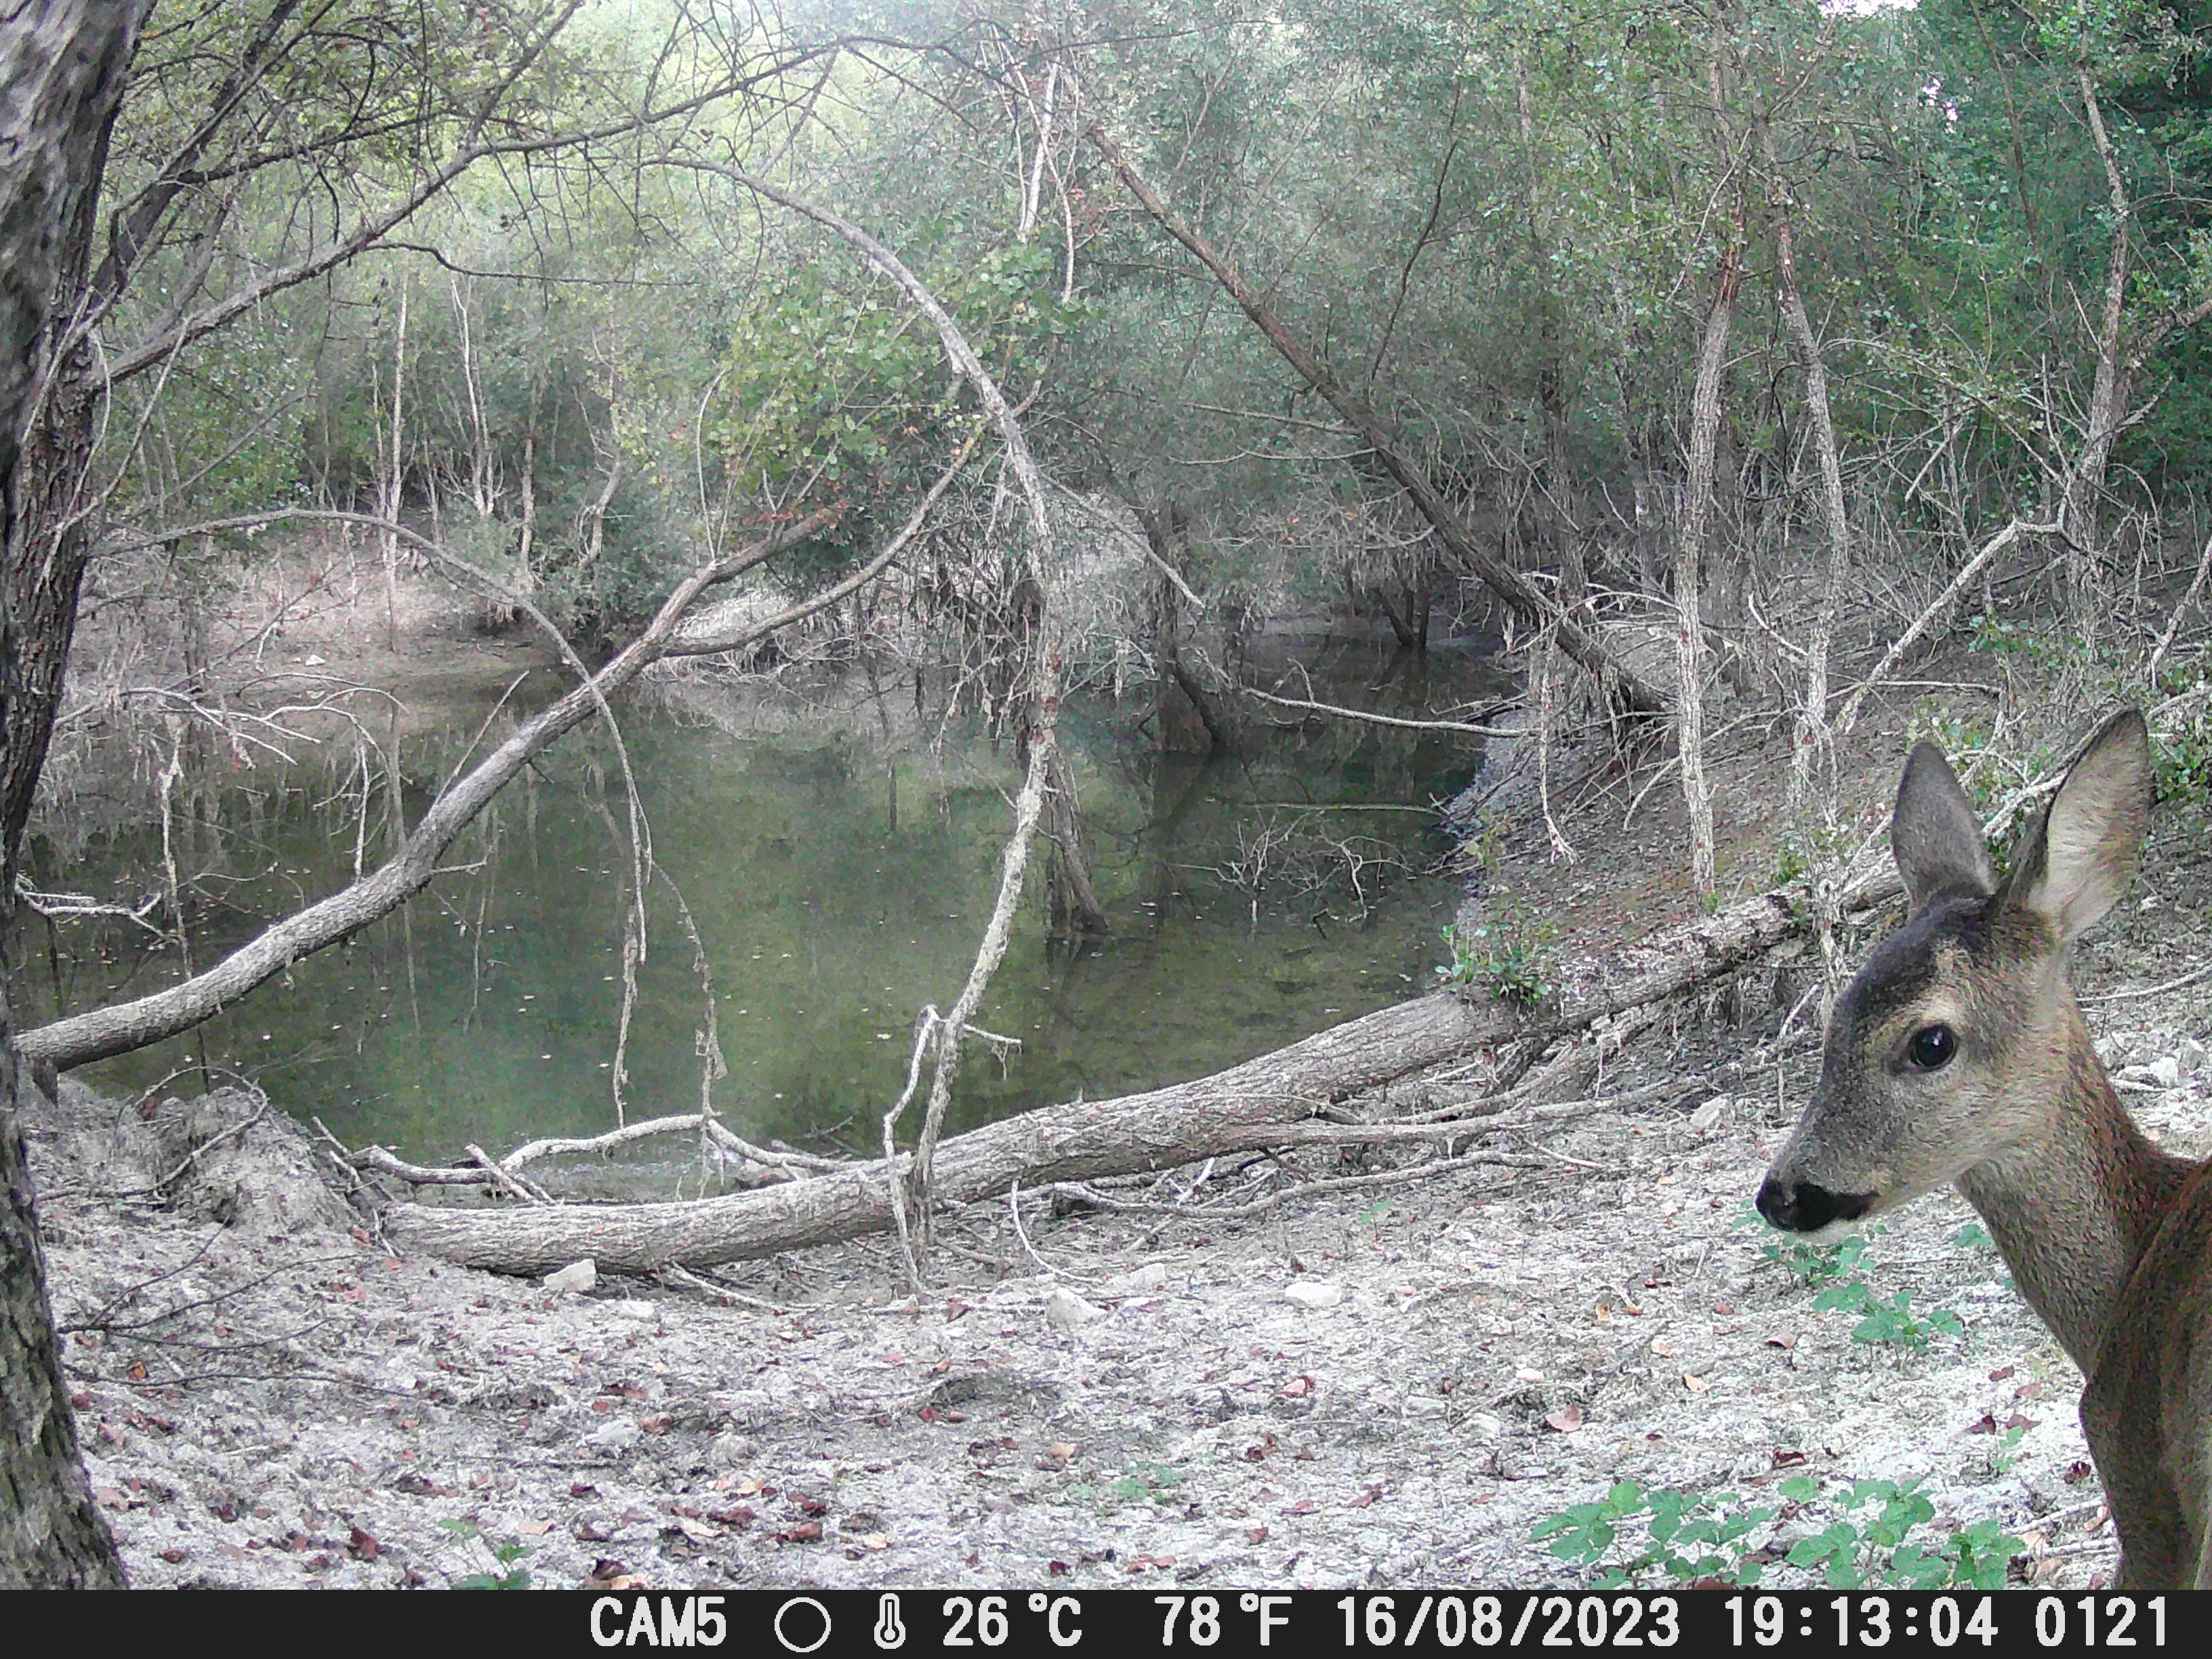
\includegraphics[width=\textwidth ,height=\textheight, keepaspectratio]{assets/TF_ACULEI_16567_DSCF0121.jpg}
    \caption{Esempio di immagine digitale scattata da una delle foto-trappole}
    \label{fig:enter-label}
\end{figure}

\subsection{Descrizione del Problema}
Si vuole creare un dataset contenente i dati di fotografie scattate automaticamente da foto-trappole 
posizionate in Umbria. Le fotografie sono state rese disponibili dal fotografo proprietario delle 
foto-trappole che le ha raccolte negli ultimi 4 anni.\\ 
Dalle fotografie si vogliono estrarre i dati principali quali la temperatura, la fase lunare, la camera 
che ha scattato l'immagine, la data e l'ora. Molto ambizioso è il riconoscimento dell'animale ritratto. 
Le fotografie possono contenere tra i meta-dati alcune di queste informazioni mentre alcune volte sono 
del tutto assenti come ad esempio la misurazione della temperature e le informazioni sulla tipologia di 
animale. La perdita di alcune informazioni nei meta-dati potrebbe essere causata da software intermedi 
che ha utilizzato il fotografo per processare le foto prima di fornirle per lo studio.\\ 
Il problema quindi è definire una serie di procedure per processare le immagini, estraendo da esse le 
informazioni rilevanti e quindi creare un dataset sul quale applicare tecniche di intelligenza artificiale 
per identificare correlazioni tra le fotografie così da offrire un'esperienza coinvolgente sull'archivio 
fotografico che le raccoglie.

\subsubsection{Motivazione del problema e rilevanza}
Il progetto aculei nasce dalla volontà del fotografo proprietario delle foto-trappole di rendere pubbliche 
le fotografie sviluppando un archivio fotografico online con forte impronta artistica. Oltre agli studi 
stilistici legati all'interazione e all'esperienza utente è stato previsto uno studio applicando 
l'intelligenza artificiale così che sia essa a guidare l'esperienza utente sull'archivio. Nel contesto del 
progetto aculei la fase descritta in questo documento rappresenta un punto molto importante per lo sviluppo 
del sistema di backend legato all'archivio fotografico.

\subsubsection{Pubblico interessato}
Le persone interessate a questo progetto sono coloro che vogliono osservare le varie fasi di creazione 
di un dataset a partire dalla raccolta dei dati fino alla realizzazione del dataset completo. Inoltre 
potrebbero essere interessati anche coloro che vogliono utilizzare il dataset per studi propri o ampliare 
e migliorare quelli al momenti svolti.

\subsubsection{Benefici di una soluzione}
Una soluzione dettagliata e ben documentata risulta sicuramente utile a definire gli step necessari alla 
creazione di un dataset nella maniera più corretta e significativa, evidenziando le difficoltà e i punti 
di forza.\\
Realizzare un dataset soddisfacente, ordinato e facilmente utilizzabile significa anche completare la 
componente che gestisce l'interazione sull'archivio \textit{aculei} attraverso il website, quindi 
creare una piattaforma di esposizione di questi contenuti fotografici, sfruttando al meglio le loro 
caratteristiche. 


\subsection{Soluzione Proposta}

\subsubsection{Approccio alla soluzione}
Per arrivare alla soluzione abbiamo eseguito diversi tenativi con molteplici tecnologie, più o 
meno sofisticate, che ci hanno restituito sia ottimi risultati che pessimi.\\
Per ottenere la soluzione ottima a cui siamo arrivati abbiamo attraversato un percorso con 
molti ostacoli, è stato fondamentale mantere la comunicazione nel gruppo. Molto spesso ci siamo 
trovati a discutere di alternative o possibili soluzione a problemi, sicuramente senza la 
interazione tra di noi non saremmo mai arrivati ad una conclusione rapidamente e avremmo 
impiegato molto più tempo ad affrontare le insidie.\\
La prima soluzione a cui avevamo pensato è stata quella di addestrare un AI con diverse immagini 
per poi cercare di ottenere un output soddisfacente ed efficiente in cui essa avrebbe dovuto 
riconoscere lo stesso animale presente nella foto. Il processo è stato piuttosto complesso e 
vedendo gli scarsi risultati abbiamo abbandonato quasi subito questa idea.\\
Dopo aver ottenuto dei risultati poco soddisfacenti ci siamo riuniti e abbiamo discusso per 
cercare una soluzione più congeniale e affine alle nostre necessità, abbiamo esplorato il 
problema pensando un po' fuori dagli schemi, oltre ad aver trovato una nuova strada abbiamo 
anche ri-organizzando il materiale a disposizione in modo da lavorare con maggiore chiarezza e 
facilità.\\
Viene deciso di proseguire per un'altra soluzione altrettanto valida e, probabilmente, più 
adeguata alla risoluzione del nostro problema. La scelta è stata quella di eseguire una 
clusterizzazione sulle immagini in modo da creare dei \textit{pool} di immagini correlate, 
viene quindi cambiata l'idea di partire dal riconoscimento dell'animale ma viene mantenuta 
l'idea di un percorso interattivo.\\
Durante la realizzazione di questa soluzione abbiamo approfondito l'uso di diversi algoritmi 
di clustering con il relativo tuning, modificando parametri, numero di clusters, tipologie di 
dati ecc.

\subsubsection{Sfide informatiche affrontate}
I problemi sono stati molteplici, affrontati durante tutta la realizzazione del progetto. Ne 
abbiamo riscontrati sia durante la prima fase in cui abbiamo cercato di allenare l'AI che durante 
la preprazione del dataset per la clusterizzazione.\\
Inizialemente il problema principale è stato quello di avere delle immagini chiare e simili in 
modo da poter insegnare quali fossero i tratti caratterstici di ciascun animale, ma essi 
risultavano troppo confusionarie e poco equiparabili, alcune erano sfocate, altre tagliate, altre 
ancora super luminose e altre totalmente buie. Un altro problema durante questa fase è stato 
quello della dimensione delle foto, esse risultavano troppo pesanti e dettagliate, quindi 
ingestibili dalla potenza di calcolo delle macchine a nostra disposizione.\\
I problemi sono proseguiti nella fase della clusterizzazione, realizzare il dataset è stato un 
lavoro lungo e macchinoso. Non avendo molta esperienza abbiamo proseguito un po a tentativi tra 
diverse metodologie. Abbiamo dovuto scegliere quali caratteristiche delle immagini tenere, quali 
fossero le più interessanti e quali quelle più facilmente reperibili in modo da avere pochi valori 
\texttt{null}. Una volta scelti i valori da studiare abbiamo dovuto capire quale fosse il metodo 
migliore per ottenerli, abbiamo testato diverse tipologie di strumenti e diverse versioni (alcuni 
OCR e lettori dettagliati di filesystem).\\
Infine abbiamo riolto diversi problemi legati alla memorizzazione dei dati in modo corretto, 
nonostante le diverse tecniche testate abbiamo avuto diversi problemi di dati inconsistenti e 
quindi abbiamo dovuto risolvere molti problemi di valori \texttt{null} all'interno del dataset. 
Talvolta abbiamo dovuto anche calcolare dei dati in modo da avere più informazioni da analizzare 
(come le stagioni o le fasi lunari), oppure convertirne alcuni in mdo da renderli sensati dal 
punto di vista della clusterizzazione (operazioni di one-hot-encoding dei dati categorici). 
Nonostante queste accortezze non siamo comunque riusciti a creare un dataset con tutti i dati che 
volevamo ma comunque alcuni sono andati persi.\\
Non sono mancate le difficoltà durante la fase di clusterizzazione, abbiamo dovuto infatti 
recuperar 

\subsubsection{Rassegna della letteratura}
Durante tutto il progetto abbiamo fatto grande uso della letteratura per recuperare informazioni 
fondamentali che ci hanno portato al suo completamento.\\
\textit{DA ESTENDERE}

\subsubsection{Divisione dei compiti nel gruppo}
Il gruppo ha lavorato abbastanza uniformemente nella realizzazione del progetto, tutti hanno 
partecipato in modo differente al completamento dello stesso.\\
Durante la stesura del codice è risultato fondamentale un approccio in cui ognuno fosse libero di 
criticare e consigliare quale fosse la soluzione ideale per lui. Ci sono state molte 
situazioni in cui ci siamo riuniti e abbiamo provato ad ideare e sviluppare delle idee per poter 
risolvere i problemi incontrati nel percorso.\\
\textit{DA ESTENDERE}

\subsubsection{Risultati ottenuti in sintesi}
Siamo riusciti ad ottenere un dataset soddisfacente con tutte le informazioni di cui necessitiamo 
e abbiamo anche già esplorato una clusterizzazione dettagliata.\\
Questi risultati ci hanno permesso di poter completare nella maniera più corretta l'interazione 
dell'archivio con il suo applicativo nel web.\\
Come dimostrato nei paragrafi successivi siamo riusciti ad effettuare una clusterizzazione che 
riteniamo più che corretta, studiando e utilizzando diverse metriche.\\
\textit{DA ESTENDERE}


\newpage
\section{Metodo Proposto}
Il metodo proposto è un insieme di differenti metodi che abbiamo testato durante l'esecuzione
per trovare quale fosse la soluzione più adeguata alle nostre esigenze.\\
Si può dire quindi che abbiamo esplorato una ampio spazio delle soluzioni per giungere a quella 
che ci sembrava essere la soluzione ideale.

\subsection{Scelta della Soluzione}
La soluzione scelta è stata quella di creare un percorso interattivo tra immagini correlate in 
grado di coinvolgere e stupire l'utente in modo dinamico. Questa soluzione è stata ottenuta 
eseguendo la clusterizzazione delle immagini raccolte.\\
Una volta collezionate, le fotografie, sono state categorizzate e indicizzate in modo da creare 
un dataset di partenza contenente tutte le informazioni reperibili più facilmente, in modo da 
poterle studiare e ordinare per poi proporre un percorso interessante all'utente finale.\\
Le soluzioni proposte non sono state poche, abbiamo provato diversi metodi e testato diverse 
tecnologie per ottenere il risultato migliore, quello che coincidesse esattamente con le nostre 
necessità di avere un sistema reattivo e sempre pronto ad essere aggiornato e migliorato con 
altre immagini e informazioni, personalizzabile dall'utente e utile sia come intrattenimento, 
quindi a scopo ludico, che interessante dal punto di vista scientifico e dell'osservazione. Per 
questo abbiamo studiato e ci siamo anche informati su quali potessero essere le correlazioni 
scientifiche con ciò che osservavamo e ciò che valutavamo, in modo da poter avere anche un 
occhio critico per poter valutare se i risultati scovati fossere corretti oppure inutili e 
sbagliati. Non essendo una materia di nostra competenza, infatti, abbiamo dovuto prestare molta 
attenzione.\\
La soluzione corretta è stata scelta anche dopo aver effettuato dell'inferenza sui dati in modo 
da osservare la distribuzione degli stessi e capire se ci fossero stati dei problemi. 

\subsubsection{Alternativi considerati e giustificazioni della scelta}
Per realizzare un percorso esplorativo tra leimmagini abbiamo fin da subito provato a realizzare 
un'AI in grado di riconoscere l'animale selvatico dall'immagine selezionta, una sorta di 
\texttt{lens} in grado di analizzare la foto e il contesto per poter tracciare quale fosse il 
soggetto e collegarla ad altre fotografie simili. L'idea è stata abbandonata piuttosto 
velocemente perchè le risorse a disposizione erano molto inferiori a quelle richieste da un 
lavoro così costoso computazionalmente parlando.\\
Per questo abbiamo optato per una soluzione più alla nostra portata e ugualmente molto 
interessante, abbiamo creato un dataset con le immagini a nostra disposizione abbiamo provato 
ad utilizzare diversi metodi di clusterizzazione con diversi parametri.\\
Dopo diverse prove e ricerche abbiamo capito che solo empiricamente e provando si può ottenere 
il risultato migliore e più adatto alle esigenze, seguendo anche la letteratura di riferimento.\\
Una volta eseguito il clustering siamo tornati sui nostri passi e abbiamo testato un metodo di 
\textit{zero-shot image classification} per poter classificare gli animali, siamo così riusciti 
ad ottenere dei risultati molto soddisfacenti.

\subsubsection{Metodologia per la misurazione delle performance}
La misurazione della performance è avvenuta tramite diversi metodi e in diversi momenti durante la 
realizzazione di questo progetto. Abbiamo sempre cercato di ottenere dei buoni risultati tenendo 
sotto controllo i dati ottenuti.\\
Per questo motivo, durante la creazione del dataset, abbiamo effettuato diversi test e diverse 
misurazioni per vedere se i dati in output fossero sensati e collezionati nel modo corretto senza 
particolari incongruenze.\\
Per il nostro progetto risulta molto complesso parlare di misurazione della performance visto che 
il risultato proposto è soggettivamente buono e non può essere valutato da parametri numerici. 
Generalmente possiamo osservare che i risultati proposti sono di nostro gradimento ma sicuramente 
possono esserci delle personalizzazioni che magari cambiano l'output in modo da ottenerne uno più 
utile al proprio scopo, magari modificando le varibili della clusterizzazione o il numero di 
clusters.\\
\textit{DA ESTENDERE / RIVEDERE}


\newpage
\section{Risultati Sperimentali}

\subsection{Dimostrazione e Tecnologie}

\subsubsection{Istruzione per la dimostrazione}
La dimostrazione che si ottiene non è altro che un percorso tra delle immagini che sono 
evidentemente correlate. Il percorso di selezione delle features, e in generale di setting di 
tutto il sistema di clusterizzazione, è avenuto dopo uno studio del dataset basato 
sull'analisi delle componenti principali (\textit{PCA}).\\ 

\subsubsection{Tecnologie e versioni usate (riproducibilità)}
Le immagini sono state scattate e raccolte maualmente da alcune foto-trappole, convertite poi in 
formato \texttt{.jpeg} e caricate su dropbox, tramite il quale è stato possibile lavorare senza 
avere con se la copia fisica delle imamgini stesse.\\ 
Per gli l'algoritmo di clustering è stato utilizzato Python (\textit{Python 3.11.7}) con alcune 
sue librerie per poter gestire e raccogliere i dati, eccone un elenco completo:
\begin{table}[h!]
    \centering
    \begin{tabular}{||l|r||l|r||}
        \hline
        \textbf{Name} & \textbf{Version} & \textbf{Name} & \textbf{Version} \\
        \hline
        easyocr & 1.7.1 & PyExifTool & 0.5.6 \\
        \hline
        ImageHash & 4.3.1 & pytesseract & 0.3.10 \\
        \hline
        matplotlib & 3.6.0 & pywaffle & 1.1.0 \\
        \hline
        numpy & 1.26.3 & Requests & 2.31.0 \\
        \hline
        opencv\_python\_headless & 4.8.1.78 & scikit\_learn & 1.0.2 \\
        \hline
        pandas & 1.4.3 & seaborn & 0.13.1 \\
        \hline
        Pillow & 10.2.0 & tqdm & 4.65.0 \\
        \hline
        transformers & 4.25.0 & & \\
        \hline
    \end{tabular}
    \caption{Python Libraries Requirements}
\end{table}

\subsection{Risultati}

\begin{table}[h!]
    \centering
% \setlength{\tabcolsep}{0.5em} % horizontal padding
% {\renewcommand{\arraystretch}{1.5} % vertical padding
    \begin{tabular}{|l|l|l|l|l|}
        \hline
        \textbf{image\_name} & \textbf{camera} & \textbf{date\_time} & \textbf{moon\_phase} & \textbf{temperature} \\ 
        \hline
        a & b & c & d & f\\
        \hline
    \end{tabular}
    \caption{???}
% }
\end{table}

Abbiamo utilizzato i dati presenti nel dataset, ottenuti dall'analisi delle immagini, per 
rappresentare al meglio i risultati ottenuti. Dopo dei processi di inferenza sono stati prodotti 
questi tre grafici, a parer nostro molto significativi al fine di comprendere la distribuzione 
dei dati a nostra disposizione nel tempo. \\
\begin{figure}[h!]
    \centering
    \includegraphics[width=\textwidth, height=\textheight, keepaspectratio]{assets/boxplot-outliers.png}
    \caption{Boxplot dei dati prima di rimuovere gli outliers}
    \label{fig:boxplot-outliers}
\end{figure}
\begin{figure}[h!]
    \centering
    \includegraphics[width=\textwidth, height=\textheight, keepaspectratio]{assets/boxplot-wout-outliers.png}
    \caption{Boxplot dei dati dopo aver rimosso gli outliers}
    \label{fig:boxplot-wout-outliers}
\end{figure}
\begin{figure}[h!]
    \centering
    \includegraphics[width=\textwidth, height=\textheight, keepaspectratio]{assets/photos-month.png}
    \caption{Numero totale di fotografie per ogni mese}
    \label{fig:photos-month}
\end{figure}
Il primo grafico è un \textit{boxplot} che rappresenta il numero di foto presenti nel dataset ad 
ogni mese, questo grafico contiene anche i dati etichettati successivamente come 
\textit{outliers}.\\ 
Successivamente abbiamo utilizzato sempre il \textit{boxplot} ma eliminando, appunto, gli 
\textit{outliers} per riuscire a farci un'idea di quante foto effettivamente potevano essere 
scattate in media dalle macchine in un mese.\\
Abbiamo utilizzato i dati senza \textit{outliers} anche per creare un \textit{grafico a barre} 
che fosse più esplitativo sul numero di foto presenti nel dataset suddivise per mese, abbiamo 
comunque osservato che ci sono dei picchi sia molto alti che molto bassi.


\subsubsection{Risultati della configurazione migliore}
Nella configurazione migliore del clustering abbiamo potuto osservare come il nostro sistema 
basato su \textit{zero-shot image classification} fosse comunque molto efficente e ci fornisse 
dei risultati abbastanza soddisfacenti, raggruppando con successo gli animali negli stessi cluster 
oppure comunque con altre immagini effettivamente simili (e quindi correlate).\\ 
\textit{DA ESTENDERE / RIVEDERE}

\subsubsection{Studio di ablazione: confronto tra configurazioni}
Effetuando la clusterizzazione all'interno del dataset abbiamo affrontato delle scelte che hanno 
comportato delle particolari configurazioni, in particolare abbiamo effettuato la \textit{PCA} e 
abbiamo esaminato i risultati ottenuti grazie alle curve descritte dal variare della varianza in 
base alle components considerate, quella del \textit{Silhouette Score} ed anceh quella del 
\textit{WCSS} (Within-Clusters Sum of Squares).\\
\textit{DA ESTENDERE / RIVEDERE}
\begin{figure}[h!]
    \centering
    \includegraphics[width=\textwidth, height=\textheight, keepaspectratio]{assets/variance-ratio.png}
    \caption{Rapporto di Varianza per numero di Components Principali}
    \label{fig:variance-ratio}
\end{figure}
\begin{figure}[h!]
    \centering
    \includegraphics[width=\textwidth, height=\textheight, keepaspectratio]{assets/elbow-silhouette.png}
    \caption{Grafico di comparazione Elbow Method - Silhouette Score}
    \label{fig:elbow-silhouette}
\end{figure}


\subsubsection{Studio di comparazione con letteratura}
\textit{DA ESTENDERE / RIVEDERE}

\newpage
\section{Discussione e Conclusioni}

\subsection{Discussione dei Risultati}
\subsubsection{Analisi delle performance rispetto alle aspettative}

\subsection{Validità del Metodo}
\subsubsection{Valutazione se il metodo rispetta le aspettative}

\subsection{Limitazione e Maturità}
\subsubsection{Limiti di applicabilità e bias}

\subsection{Lavori Futuri}
\subsubsection{Proposte per avanzare il progetto}

\newpage
\paragraph{Acknowledgements} Si ringrazia Tobia Faverio per aver reso possibile lo sviluppo di 
questo progetto fornendo le fotografie e per la sua idea che ha dato vita ad \textit{aculei}.

\newpage
\printbibliography

\end{document}